\chapter{Gaussian Blur}
	Gaussian Blur.

\section{Error}

	\begin{dfn}\index{convolution!one-dimensional}
		Let $f$ and $g$ belong to $L^1(\mathbb{R})$. The \emph{convolution}, $f*g$ defined as:
		\begin{equation}\label{def_convolve_1D}
			(f*g)(x)=\int_{-\infty}^\infty f(x-\tau)g(\tau)d\tau
		\end{equation}
	\end{dfn}

	In the context of image analysis we are dealing with real-valued functions that are generally bounded (by intensity such as 0 to 255). So these functions behave nicely and therefore we can assume the covolution exists. For more information on the existance of the convolution see Yeh \cite{yeh_1}.

	\begin{figure}[!htb]
			\centering
			\subfigure[$f(x)$]{
				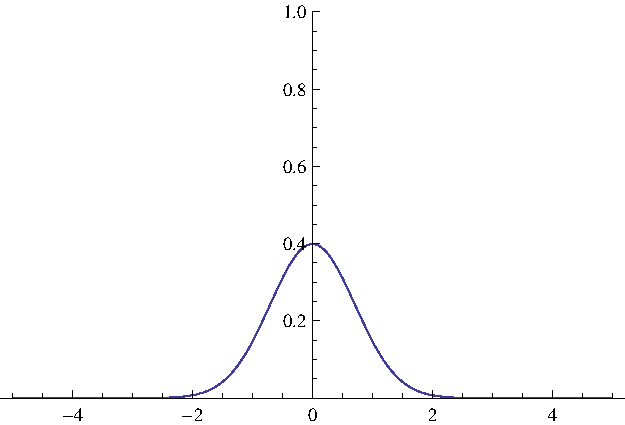
\includegraphics[width=2in]{graph_01}}
			\subfigure[$g(x)$]{
				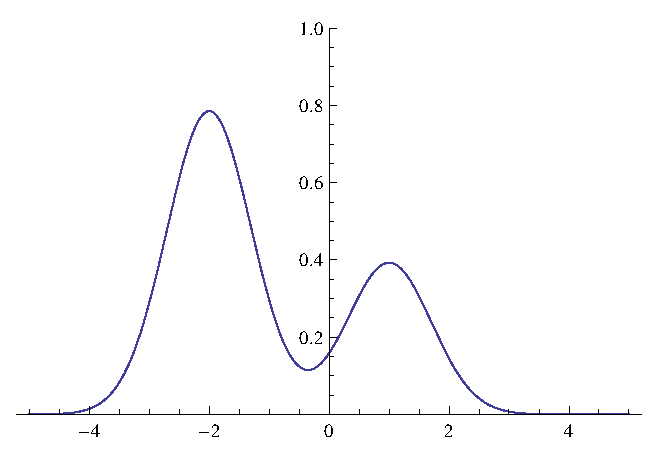
\includegraphics[width=2in]{graph_02}}
			\subfigure[$f(x-2)g(x)$]{
				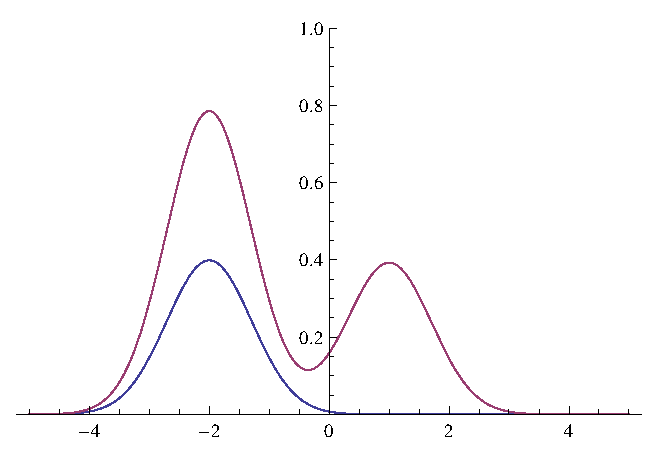
\includegraphics[width=2in]{graph_03}}
			\subfigure[$f(x-1)g(x)$]{
				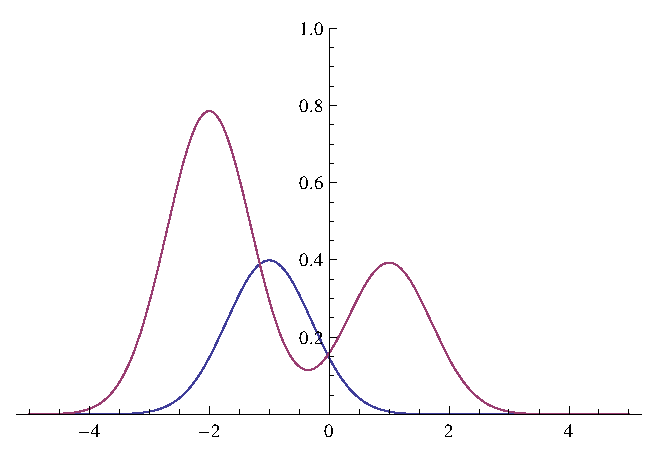
\includegraphics[width=2in]{graph_04}}
			\subfigure[$f(x-0)g(x)$]{
				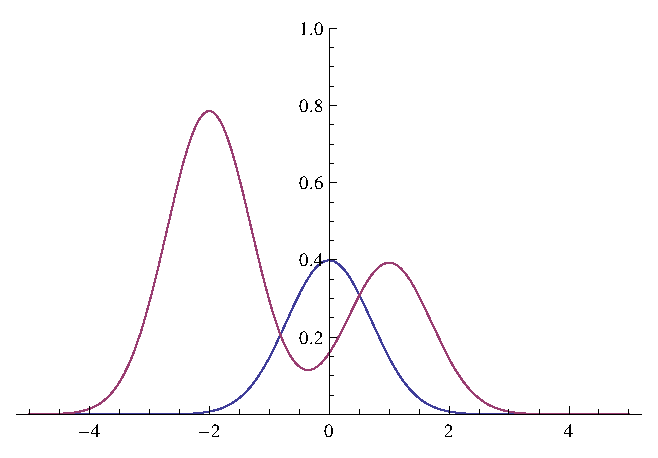
\includegraphics[width=2in]{graph_05}}
			\subfigure[$f(x+1)g(x)$]{
				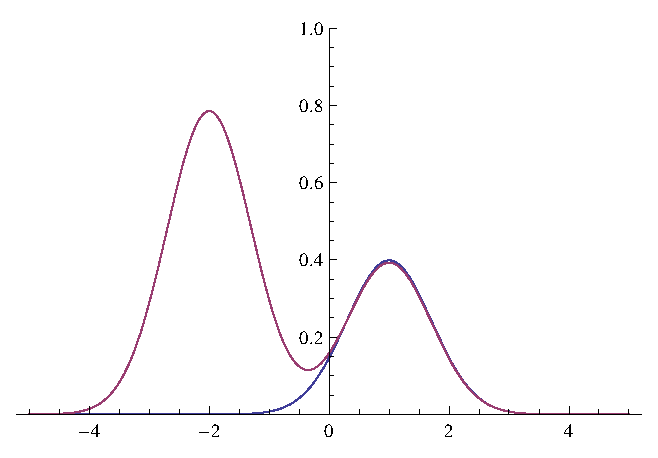
\includegraphics[width=2in]{graph_06}}
			\subfigure[$f(x+2)g(x)$]{
				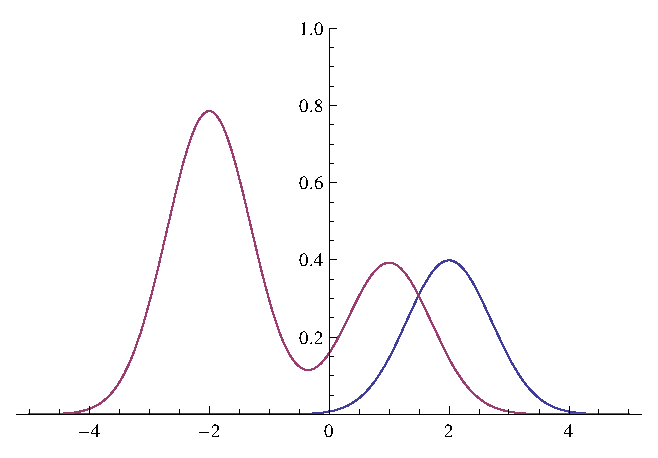
\includegraphics[width=2in]{graph_07}}
			\subfigure[$f*g$]{
				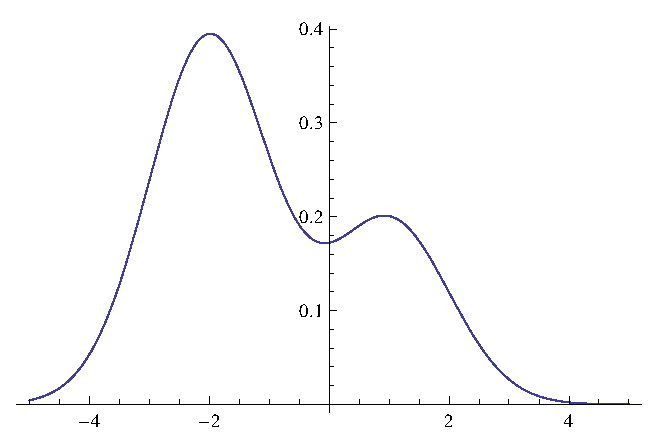
\includegraphics[width=2in]{graph_08}}
			\caption{One-dimensional convolution example}
			\label{fig_convolution}
	\end{figure}
	\clearpage
	
	The convolution has many properties that are useful. 
	\begin{prop}
		The convolution has the following properties (prove).
		\begin{enumerate}
		\item $f*g=g*f$ (commutative)
		\item $f*(g*h)=(f*g)*h$ (associative)
		\item $f*(g+h)=(f*g)+(f*h)$ (distributive)
		\item $a(f*g)=(af*g)=(f*ag)s$ for $a\in\mathbb{R}$ (associativity with scalar multiplication)
		\end{enumerate}
	\end{prop}
	\begin{proof}\hspace{10mm}
		\begin{enumerate}
		\item Substitute $\kappa=x-\tau$, $d\kappa=-d\tau$ into the defintion of convolution so \mbox{$(f*g)(x)=-\int_{\infty}^{-\infty}f(\kappa)g(x-\kappa)d\kappa$}. Switching the limits of integration and the order of $f$ and $g$ we have \mbox{$(f*g)(x)=\int_{-\infty}^\infty g(x-\kappa)f(\kappa)d\kappa$}. Rename the variable of integration $\kappa$ back to $\tau$ (this rename doesn't change anything) and we get \mbox{$(f*g)(x)=\int_{-\infty}^\infty g(x-\tau)f(\tau)d\tau=(g*f)(x)$}
		\item Using the defintion
			\begin{equation*}\begin{array}{rl}
				(f*(g*h))(x)&=\int_{-\infty}^\infty f(x-\tau)(g*h)(\tau)d\tau\\
				&=\int_{-\infty}^\infty f(x-\tau)\left[ \int_{-\infty}^\infty g(\tau-\kappa)h(\kappa)d\kappa\right]d\tau\\
				&=\int_{-\infty}^\infty\int_{-\infty}^\infty f(x-\tau)g(\tau-\kappa)h(\kappa)d\kappa d\tau.
			\end{array}\end{equation*}
			By Fubini's theorem we can switch the order of integration so
			\begin{equation*}\begin{array}{rl}
				(f*(g*h))(x)&=\int_{-\infty}^\infty\int_{-\infty}^\infty f(x-\tau)g(\tau-\kappa)h(\kappa)d\tau d\kappa\\
				&=\int_{-\infty}^\infty f(x-\tau)\left[\int_{-\infty}^\infty g(\tau-\kappa)h(\kappa)d\tau\right]d\kappa.
			\end{array}\end{equation*}
			Since we are working in a translation invarient metric we have
			\begin{equation*}\begin{array}{rl}
				(f*(g*h))(x)&=\int_{-\infty}^\infty f(x-\tau)\int_{-\infty}^\infty[g((\tau+\kappa)-\kappa)h(x-(\tau+\kappa))d\tau]d\kappa\\
				&=\int_{-\infty}^\infty f(x-\tau)\int_{-\infty}^\infty[g(\tau)h((x-\kappa)-\tau))d\tau]d\kappa\\
				&=\int_{-\infty}^\infty f(x-\tau)(g*h)(x-\kappa)d\kappa\\
				&=((f*g)*h)(x).
			\end{array}\end{equation*}
		\item
			\begin{equation*}\begin{array}{rl}
				(f*(g+h))(x)&=\int_{-\infty}^\infty f(x-\tau)(g(\tau)+h(\tau))d\tau\\
				&=\int_{-\infty}^\infty f(x-\tau)g(\tau)+f(x-\tau)h(\tau))d\tau\\
				&=\int_{-\infty}^\infty f(x-\tau)g(\tau)+\int_{-\infty}^\infty f(x-\tau)h(\tau))d\tau\\
				&=(f*g)(x)+(f*h)(x).
			\end{array}\end{equation*}
		\item
			\begin{equation*}\begin{array}{rl}
				a(f*g)(x)&=a\int_{-\infty}^\infty f(x-\tau)g(\tau)d\tau\\
				&=\int_{-\infty}^\infty af(x-\tau)g(\tau)d\tau\\
				&=(af*h)(x).
			\end{array}\end{equation*}
			The other equality is proved exactly the same way.
		\end{enumerate}
	\end{proof}
	
	Differentiation.
	\begin{equation*}\index{convolution!derivative 1D}
		\frac{d}{dx}(f*g)=(\frac{df}{dx}*g)(x)=(f*\frac{dg}{dx}g)(x)
	\end{equation*}
	
	
\section{Two-Dimensional Convolution}
	In two dimensions:
	\begin{dfn}\index{convolution!two-dimensional}
		Let $f$ and $g$ belong to $L^2{\mathbb{R^2}}$. The convolution, $(f*g)$ defined as:
		\begin{equation}\label{def_convolve_2D}
			(f*g)(x,y)=\int_{-\infty}^\infty\int_{-\infty}^\infty f(x-\tau,y-\kappa)g(\tau,\kappa)d\tau d\kappa
		\end{equation}
	\end{dfn}
	
	Differentiation in two variables.
	\begin{equation*}\index{convolution!derivative 2D}
		\frac{\partial}{\partial x}(f*g)=\frac{\partial f}{\partial x}*g=f*\frac{\partial g}{\partial x}
	\end{equation*}
	\begin{equation*}
		\frac{\partial}{\partial y}(f*g)=\frac{\partial f}{\partial y}*g=f*\frac{\partial g}{\partial y}
	\end{equation*}

\section{Discrete Convolution}
	We will only examine the two dimensional case.
	\begin{dfn}
		Let $f$ and $g$ be functions ...?
		\begin{equation*}\index{convolution!two-dimensional discrete}
			(f\otimes g)(x,y)=\sum_{i=0}^{M-1}\sum_{j=0}^{N-1}f(i-x,j-y)g(i,j).
		\end{equation*}
	\end{dfn}

\section{Convolution Implementation}

	\lstinputlisting{test.c}

\section{One-Dimensional Correlation}
	Correlation
	\begin{dfn}
		
	\end{dfn}
